\cotefile{89}
\scanpage{2}
% L1, top right
\begin{flushright}
les \unsure{ensembles|ensemble} 3-3
\end{flushright}
% archive sheet number: 1

\scanpage{3}\mspage{I}
% L1
Soit $H=(S,A,R)$ un hexagone combinatoire

\figure{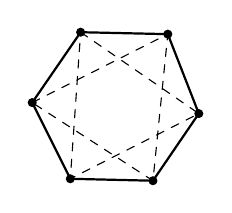
\begin{tikzpicture}[line cap=round,line join=round,scale=.82]
\coordinate (a) at (-.70,1.16); \coordinate (b) at (.65,1.13);
\coordinate (c) at (1.13,-.10); \coordinate (d) at (.42,-1.14);
\coordinate (e) at (-.86,-1.11); \coordinate (f) at (-1.45,.07);
\draw[thick] (a)--(b)--(c)--(d)--(e)--(f)--cycle;
\draw[dashed] (a)--(c)--(e)--cycle (f)--(b)--(d)--cycle;
\foreach \v in {a,b,c,d,e,f}{\fill (\v) circle (2pt);}
\end{tikzpicture}}

% L2–6
Il lui correspond

a) $\omega_H\in\mathrm{Ens}_2$ \unsure{l'ens|l'une} des deux orientations

b) Un torseur $S$ sous $\deleted{\unsure{\mathbb Z/6\mathbb Z\wedge\omega_H|\mathbb Z/6\mathbb Z\wedge\omega_H\simeq}\;\unsure{\mathbb Z/3\mathbb Z\wedge\omega_H}}$
\[
\mathbb Z/6\mathbb Z\wedge\omega_H \simeq
(\mathbb Z/3\mathbb Z\wedge\omega_H)\times
\underbrace{(\mathbb Z/2\mathbb Z\wedge\omega_H)}_{\mathbb Z/2\mathbb Z}
\]
ou ce qui revient au $=$, une paire de deux torseurs.

% L7–10
b$_1$) Un torseur sous $(\mathbb Z/3\mathbb Z\wedge\omega_H)$ i.e. un \deleted{tri} élément
\[
\left\{\begin{aligned}
&\Delta\in\mathrm{Ens}_3\quad\text{avec iso}\\
&\omega_\Delta\simeq\omega_H
\end{aligned}\right.
\]
\margin{\uline{NB} a) et b$_1$) \unsure{équiv. à|équivaut à} : la donnée de $\Delta\in\mathrm{Ens}_3$}
% slanted
\margin{Le groupoïde des hexagones combinatoires est équivalent à la catégorie $(\mathrm{Ens})_3\times(\mathrm{Ens})_2$}
b$_2$) un ens $\unsure{\tau|T}$ à deux éléments

% L11–19
Alors $\Delta$ s'interprète comme l'ens des \deleted{\unsure{deux}}\inserted{trois} diagonales\unsure{,} de $H$, et $\tau$ comme l'ens des deux triangles inscrits. On récupère $\deleted{H}S$ par un iso. can.
\[
S\simeq\Delta\times\tau
\]
(un sommet est connu quand on connaît le triangle inscrit et la diagonale \unsure{que il|qu'il} détermine, et inversement, ceux-ci peuvent être donnés arbitrairement -- )

% L20–22
Notons que cette décomposition implique
\[
S\simeq\coprod_{i\in\tau}S_i\qquad\text{avec}\quad
\begin{aligned}
&\operatorname{card}\tau=2\\
&\operatorname{card}S_i=3\qquad\forall i\in\tau
\end{aligned}
\]
% archive sheet number: 2

\scanpage{4}
% L1–5
en posant
\[
S_i=\Delta\times\{i\}\qquad,
\]
et on a un iso. canonique $\omega_{S_i}\simeq\omega_\Delta$ pour \unsure{tt|$\forall$} $i\in\unsure{\tau|T}$, d'où
\[
\bigwedge_{i\in\tau}\omega_{S_i}\simeq\unsure{\mathbb{1}|\underline{1}}.
\quad\text{(torseur unité sous $\mathbb Z/2\mathbb Z$)}
\]

% L6–12
Considérons la structure \deleted{donnée} sur un ens $S$ de card $6$ \unsure{donnée|donné} par une partition
\[
S=\coprod_{i\in\tau}S_i
\]
du type $(3,3)$, et un \inserted{\unsure{syst. trans.} d'}\unsure{isom|isom.} entre les $\omega_{S_i}$ i.e. un isom
\[
\bigwedge_{i\in\tau}\omega_{S_i}\simeq\mathbb{1}.\tag*{$(*)$}
\]

% L13–15
\deleted{Considérons les} Le groupe des \unsure{autom.|automorph.} de cette structure est d'ordre $36$ (on a en effet
\diagram{\begin{tikzcd}[ampersand replacement=\&,column sep=1em,row sep=1.1em]
\&1\arrow[d]\\
1\arrow[r]\&G'\arrow[r]\arrow[d]\&G\arrow[r]\&{\unsure{\mathfrak S|\mathfrak G}_{\tau}}\arrow[d,equal]\arrow[r]\&1\&{\big)}\\
\&{\displaystyle\mathop{\deleted{\mathfrak S}\mkern-14mu\prod}\limits_{i\in\tau}\mathfrak S_{S_i}}\arrow[d,"{\prod_{i\in\tau}\mathrm{sg}_i}"]\&\&{\mathbb Z/2\mathbb Z}\\
\&{\mathbb Z/2\mathbb Z}\arrow[d]\\
\&1
\end{tikzcd}}

% L16–17
\deleted{Le sous-groupe}

Une structure hexagonale subordonnée à la
% archive sheet number: 3

\scanpage{5}
% L1–6
structure envisagée équivaut à la donnée de l'\uline{antipodisme} correspondant $\sigma=\sigma_H$ à cette structure $H$, qui \deleted{\unsure{doit}} \inserted{est} un autom \inserted{involutif} de la structure envisagée, induisant la transposition de $\unsure{\tau|T}$ i.e. échangeant entre eux les deux ens. $S_i$
% slanted
\margin{\deleted{en effet, tout élément d'ordre $2$ de \unsure{$G$}}}
% slanted
\margin{il faut exiger de plus que $\sigma$ opère trivialement sur le $\omega$ (défini comme le ``$\omega$ commun'' des $\omega_{S_i}$ $(i\in\tau)$) \unsure{$\Leftrightarrow$|$\rightleftarrows$} il y en a trois autres inv. qui induisent \deleted{\unsure{l'aut.}} la transp. antipodique de \unsure{$\tau$} \uline{et} de $\omega$, ils correspondent aux éléments $\unsure{t_\sigma|t_{\sigma'}}$ de $\bigwedge_{i\in\tau}S_i$ (produit contracté sous $\unsure{\Gamma_\omega|\mathscr T_\omega}=\mathbb Z/3\mathbb Z\wedge_{\pm1}\omega$)}
-- il y en a exactement $3$ correspondant (pour le choix d'un $i\in\tau$ \unsure{fixé}) aux trois \unsure{isom|isoms}
\[
S_i\simeq S_j\qquad(j\in\tau,\ j\ne i)
\]
qui ``conservent l'orientation''\unsure{)} i.e. induisent $\omega_{S_i}\simeq\omega_{S_j}$ l'iso. donné grâce à \unsure{$(*)$|$(A)$}. \deleted{Soit}

% L13–20
Alors l'ens $G_H$ des autom de $H=H_\sigma$ est le centralisateur de $\sigma$ -- $G_H$\inserted{$=Z(\sigma)$} est d'indice $3$ dans $G$, il est non distingué\inserted{ et en fait est son propre normalisateur}, ses trois conjugués correspondent aux trois conjugués de $\sigma$, qui sont les trois ``antipodismes'' de $G$, \unsure{correspondants|correspondant} aux trois structures hexagonales subordonnées à la structure ``trihexagonale'' envisagée.

% archive sheet number: 4
% L21–22
Considérons le sous-groupe (invariant) \inserted{$G'$} de $\deleted{\unsure{G'}}G$ engendré par \unsure{l'ens|l'un|l'ens.} $I$ des trois anti%
\scanpage{6}%
% L1–4; continuation of anti- at the foot of scan 5
podismes $\sigma_i$, on vérifie que pour
\[
I=\{i,j,k\}
\]
on a
\[
\sigma_k=\sigma_i\sigma_j\sigma_i
\]
% L5–8
\deleted{\unsure{d'où|donc}}\unsure{ce|donc} qui \inserted{\unsure{donc|nous|peut}} \unsure{exige|exiger} (en faisant une permutation circulaire, donc
\[
\begin{aligned}
\sigma_i&=\sigma_j\sigma_k\sigma_j
=\sigma_{\deleted{\unsure{i}}j}(\sigma_i\sigma_j\sigma_i)\sigma_j
\qquad\deleted{\text{i.e.}}\\
(\sigma_i\sigma_j)^3&=1
\end{aligned}
\]

% L9–15
On \deleted{constate que $\unsure{G|G'}$ est le sous-groupe présenté} \inserted{voit que $G'$ opérant sur} $I$ donne un iso \deleted{par}
\[
\deleted{\sigma_i^2=1\qquad(i\in I)}
\]
\[
\deleted{\unsure{\sigma}}\qquad G'\xrightarrow{\sim}\unsure{\mathfrak S|\mathfrak G}_I
\]
avec $\sigma_i$ correspondant à la transposition de $I$ d'indice $i$ -- $G'$ est présenté par les gén. $\sigma_i$ \inserted{$(i\in I)$} et les \inserted{$3+6=9$} relations
\[
\sigma_i^2=1\qquad \sigma_k=\sigma_i\sigma_j\sigma_i\qquad
\text{(si $I=\{i,j,k\}$,}
\]

% L16–19
ou encore (pour $i,j\in I$ fixés, $i\ne j$ \deleted{\unsure{$j$|)}}, posant \unsure{ici} $\sigma=\sigma_i,\sigma'=\sigma_j$)
\[
\deleted{\sigma_i^2=\sigma_j^2=}
\]
\[
\sigma^2=\sigma'{}^2=(\sigma\sigma')^3=1\quad.
\]

% L20–21
Quel est le groupe quotient $G/G'$ (d'ordre $6$) ? Notons que \deleted{\unsure{les}}\unsure{la|les} \inserted{donnée} \deleted{\unsure{str.}} de $(S_i)_{i\in\unsure{\tau|T}}$
% archive sheet number: 5

\scanpage{7}
% L1–5
et de $\bigwedge_{i\in\unsure{\tau|T}}\omega_{S_i}=\unsure{\mathbb{1}|\underline{1}}$ équivaut à la donnée d'un ens à deux éléments $\omega$ (la ``valeur commune'' des $\omega_{S_i}$ identifiés par le syst. transitif d'iso $\bigwedge_{i\in\tau}\omega_{S_i}\simeq\mathbb{1}$) et une famille de \uline{torseurs} $S_i$ $(i\in\tau)$ sous $\mathbb Z/3\mathbb Z\wedge_{\pm1}\omega=\Gamma_\omega$

% L6–10
Considérons alors le \inserted{$\Gamma_\omega$-}torseur :
\[
\deleted{\unsure{\lambda}}T=\deleted{\prod_{i\in\tau}}\bigwedge_{i\in\tau}S_i
\]
alors $G$ opère sur $(\Gamma_\omega,T)$ je dis que $G'$ y opère trivialement. En effet, un antipodisme $\sigma$ induisant $S_i\overset{u}{\simeq}S_j$ et $S_j\overset{u^{-1}}{\simeq}S_i$ induit
\[
S_i\wedge S_j\xrightarrow{\sim}S_j\wedge S_i
\overset{\mathrm{sym}}{\simeq} S_i\wedge S_j
\qquad (x\wedge y)\longrightarrow(u^{-1}y\wedge ux)
\]

% L11–15
\deleted{Or si \unsure{$u'x$|$ux$}} Fixons $a\in S_i$, posons $ua=b\in S_j$, on a donc pour $\gamma,\gamma'\in\Gamma_\omega$\qquad $x=\gamma a,y=\gamma'b$
\[
\sigma(\underbrace{\gamma a\wedge\gamma'b}_{\gamma\gamma'\,a\wedge b})
=(\underbrace{\deleted{\unsure{v|u}}u^{-1}\gamma'b}_{\gamma'a})\wedge
\underset{\gamma b}{(u\gamma a)}
=\deleted{\unsure{\gamma\gamma'}}\underset{\gamma'\gamma\,a\wedge b}{\gamma'a\wedge\gamma b}
\]

% L16–21
Ainsi $G/G'$ opère sur \deleted{\unsure{$T,\omega$}}$(\Gamma_\omega,T)$. Mais $T$ se réalise \inserted{\unsure{canoniqt|canoniquement|canonique}} comme l'ens des \inserted{$3$} autom involutifs $\unsure{\alpha|\deleted{\alpha_\psi}}$ de $S=\coprod_{i\in\tau}S_i$ tels que $\alpha$ induise la transposition de $\tau$ \uline{et} de $\omega$, et on vérifie que $\alpha_t$ conjugue $\alpha_{\unsure{t'|j'}}$ en $\alpha_{\unsure{t''|j''}}$ (en fait, on l'a déjà fait \ldots)
% archive sheet number: 6

\scanpage{8}
\begin{center}\rule{1.5cm}{.4pt}\\[-.9ex]\hspace{.25cm}\rule{1.25cm}{.4pt}\end{center}
% L1–5
Soit $S$ \deleted{\unsure{d'un|de}}de cardinal $6$ muni d'une partition \inserted{$R$} de type $(3.3)$, $\unsure{\tau|T}$ l'ens de ses deux classes, $S_i$ $(i\in\tau)$ ses deux classes. Soit $\unsure{\mathcal G|g}$ le groupe des autom de $S$, donc
\diagram{\begin{tikzcd}[ampersand replacement=\&,column sep=1em,row sep=.4em]
1\arrow[r]\&{\displaystyle\prod_{i\in\tau}\unsure{\mathfrak S|\mathfrak G}_{S_i}}\arrow[r]\&\mathcal G\arrow[r]\&\mathfrak S_\tau\arrow[r]\arrow[d,equal]\&1\\
\&\&\&{\mathbb Z/2\mathbb Z}
\end{tikzcd}}

% L7–11
$\mathcal G$ d'ordre $72$. Soit $S'\subset\mathcal G$ l'ens des éléments \uline{involutifs} de $\mathcal G$ au dessus de l'élément $\ne1$ de $\mathfrak S_\tau$, i.e. l'ens des scindages de l'ext. précédente.

% L12–17
Pour $i\in\tau$ fixé, il est en corr. $1$-$1$ avec $\deleted{\unsure{\mathrm B|\mathrm I}}\operatorname{Isom}(\mathfrak S_i,\mathfrak S_{\deleted{\unsure{j}}\bar i})$ où $\substack{\bar i\in\tau\\\bar i\ne i}$, ou encore il est en corr. $1$-$1$ avec l'ens des corr. bijectives entre $(\mathfrak S_i)_{i\in\tau}$, i.e. des $\Gamma\subset\prod_{i\in\tau}S_i$ \unsure{telles|tels} que \inserted{$\forall i\in\tau$} $\Gamma\unsure{\mathord{-}|\to} S_i$ soit bij.
% archive sheet number: 7

\scanpage{9}
% L1–7
C'est un ens qui a $\unsure{6|\sigma}$ éléments, et on a une \deleted{bijection} surjection
\[
\begin{aligned}
S'&\longrightarrow\unsure{\tau'|T'}\overset{\text{déf}}{=}\bigwedge_i\omega_{S_i}\\
&\hspace{4em}\text{(noté $\omega$ précédemment)}
\end{aligned}
\]
\deleted{\unsure{d}}qui est de degré $3$. Donc $S'$ est \unsure{égalemt|également} un ens. muni d'une partition de type $(3,3)$.

% L8–12
La donnée d'une structure \unsure{hexagonale|hexagonal} équivaut à celle d'une structure $(S,R)$, et d'un $s\in S'$ -- celle d'un hexagone et d'un sommet dessus, à un
% archive sheet number: 8

\scanpage{10}\mspage{II}
% L1–4
Soit $V$ un \deleted{\unsure{espace}}plan vectoriel sur $\mathbb F_3$. La droite projective $P(V)$ a quatre éléments i.e. $V$ \deleted{\unsure{a}}\inserted{contient} quatre droites vectorielles -- donnons nous une paire \inserted{$\unsure{\tau|T}$} de droites de $V$ $(D_i)_{i\in\tau}$. On a donc
\[
V=\mathop{\deleted{\prod}\mkern-15mu\bigoplus}_{i\in\tau}D_i\simeq\prod_{i\in\tau}D_i
\tag*{(1)}
\]
% L6–8
Considérons la paire complémentaire $\tau'=P(V)\smallsetminus\tau$, \deleted{\unsure{elle}}\unsure{on} a donc aussi
\[
V=\bigoplus_{i\in\tau'}D_i\simeq\prod_{i\in\tau'}D_i
\tag*{(2)}
\]
% L9–15
Notons les relations
\[
\left\{\begin{aligned}
\tau'&\simeq\bigwedge_{i\in\tau}D_i^*\\
\tau&\simeq\bigwedge_{i\in\tau'}D_i^*
\end{aligned}\right.
\tag*{(3)}
\]
l'application
\[
\prod_{i\in\tau}D_i^*\longrightarrow\tau'
\]
qui définit $\bigwedge_{i\in\tau}^{i}D_i^*\unsure{\mathord{-}|\to}\tau'$ étant
\[
(u_i)_{i\in\tau}\longrightarrow\mathbb F_3\mathbin{\cdot}
\left(\sum_{i\in\tau}u_i\right)\quad.
\tag*{(4)}
\]
% L16–21
Si $P$ est un $V$-torseur, i.e. un \deleted{\unsure{espace|plan}}\inserted{plan} affine sous $\mathbb F_3$ admettant $V$ comme groupe de translations, \unsure{alors|donc} les formules (1) et (2) définissent respectivement deux décompositions de $P$ en produits
\[
P\unsure{=|\simeq}\prod_{i\in\tau}P_i\unsure{\mathord{-}|\mathord{.}},\qquad
P\simeq\prod_{i\in\tau'}P_i\unsure{.|'}
\tag*{(5)}
\]
% archive sheet number: 9

\scanpage{11}
% L1–3
\deleted{\unsure{ce qui|où pour}}\inserted{où} pour tout $i\in\unsure{\tau|T}\amalg\tau'\deleted{\unsure{P}}=P(V)$, $P_i$ est un $D_i$-torseur, défini par
\[
P_i=P/D_{\bar i}=P\wedge_V(D_i\simeq V/D_{\bar i})
\tag*{(6)}
\]
% L4–9
où $i\mapsto\bar i$ est l'\deleted{\unsure{élément}}\inserted{involution} de $P(V)$ qui \deleted{est} correspond à sa partition de type $(2,2)$ $\{\tau,\tau'\}$, qui dans $\tau$ et dans $\tau'$ se réduit à la transposition dans ces ensembles. Ainsi, l'ensemble $P$, de cardinal $9$, est muni, via
\[
P\simeq\prod_{i\in\tau}P_i
\tag*{$(*)$}
\]
% L10–18
\deleted{de}d'\deleted{deux}\inserted{une \deleted{\unsure{autre}}paire de} partitions de type $(3,3,3)$, \unsure{indexée|indexées} par $\tau$, ces partitions étant ``d'équerre'', en ce sens que l'application canonique \inserted{\unsure{ces|cs|de}} de $P$ sur le produit des deux ens. quotients correspondants est bijective, ce qui signifie aussi que pour tte classe de l'une et toute classe de l'autre, l'intersection a exactement un élément (il suffit de supposer qu'elle est tjrs non vide; ou qu'elle a tjrs au plus un élément\ldots). Et ce même ensemble $P$ est muni d'une deuxième paire (distincte de la première) de partitions de type $(3,3)$, \inserted{``en équerre'', \unsure{indexée|indexées} par $\tau'$,} correspondant à la décomposition
\[
P\simeq\prod_{i\in\tau'}P_i
\tag*{$(*')$}
\]
% archive sheet number: 10

